\section{Sequential MNIST}

\subsection{Task and evaluation criteria}
The simple function task is a purely synthetic task, that does not require a deep network. As such it does not test if an arithmetic layer inhibits the networks ability to be optimized using gradient decent.

The sequential MNIST task takes the numerical value of a sequence of MNIST digits and applies a binary operation recursively. Such that $t_i = Op(t_{i-1}, z_t)$, where $z_t$ is the MNIST digit's numerical value.

The performance of this task depends on the quality of the image-to-scalar network and the arithmetic layer's ability to model the scalar. We use mean-square-error (MSE) to evaluate joint image-to-scalar and arithmetic layer model performance. To determine an MSE threshold from the correct prediction we use an empirical baseline. This is done by letting the arithmetic layer be solved, such that only the image-to-scalar is learned. By learning this over multiple seeds an upper bound for an MSE threshold can be set. In our experiment we use the 1\% one-sided upper confidence-interval, assuming a student-t distribution.

Similar to the simple function task we use a success-criteria as reporting the MSE is not interpretable and models that do not converge will obscure the mean. Furthermore, because the operation is applied recursively, natural error from the dataset will accumulate over time, thus exponentially increasing the MSE. Using a baseline model and reporting the successfulness solves this interpretation challenge.

\subsection{Addition of sequential MNIST}

Figure \label{fig:sequential-mnist-sum} shows results for sequential addition of MNIST digits. This experiment is identical to the MNIST Digit Addition Test from \citet[section 4.2]{trask-nalu}. The models are trained on a sequence of 10 digits and evaluated on sequences between 1 and 1000 MNIST digits.

Note that the NAU model includes the $R_z$ regularizer, similarly to the ``Multiplication of sequential MNIST'' experiment in section \ref{section:results:cumprod_mnist}. To provide a fair comparison, a variant of $\mathrm{NAC}_{+}$ that also uses this regularizer is included, this variant is called $\mathrm{NAC}_{+, R_z}$. Section \ref{sec:appendix:sequential-mnist-sum:ablation} provides an ablation study of the $R_z$ regularizer.

\begin{figure}[h]
\centering
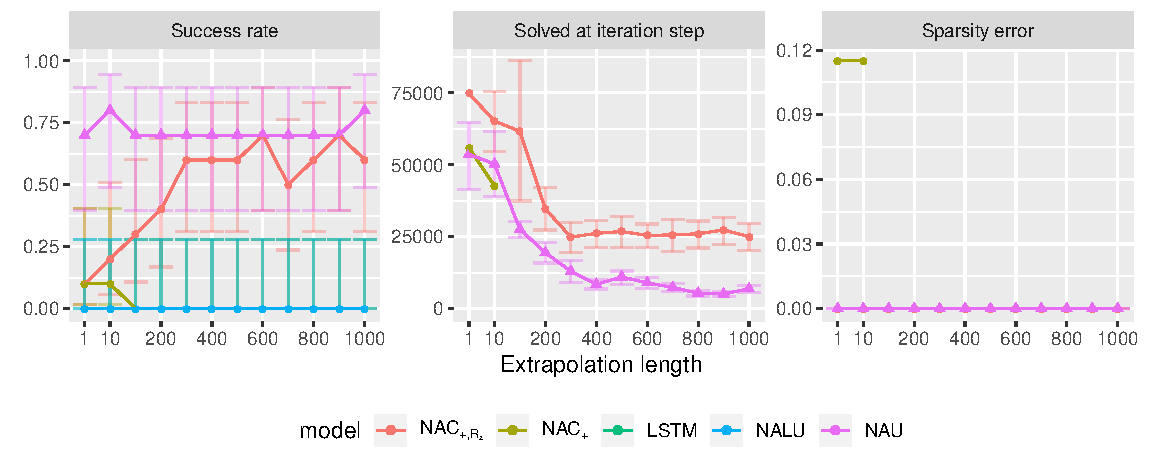
\includegraphics[width=\linewidth,trim={0 0.5cm 0 0},clip]{paper/results/sequential_mnist_sum_long.pdf}
\caption{Shows the ability of each model to learn the arithmetic operation of addition and backpropagate through the arithmetic layer in order to learn an image-to-scalar value for MNIST digits. The model is tested by extrapolating to larger sequence lengths than what it has been trained on. The NAU and $\mathrm{NAC}_{+,R_z}$ models use the $\mathrm{R}_z$ regularizer from section \ref{section:results:cumprod_mnist}.}
\label{fig:sequential-mnist-sum}
\end{figure}

\subsection{Sequential addtion without the \texorpdfstring{$\mathrm{R}_z$}{R\_z} regularizer}
\label{sec:appendix:sequential-mnist-sum:ablation}

As an ablation study of the $\mathrm{R}_z$ regularizer, figure \ref{fig:sequential-mnist-sum-ablation} shows the NAU model without the $\mathrm{R}_z$ regularizer. Removing the regularizer causes a reduction in the success-rate. The reduction is likely larger, as compared to sequential multiplication, because the sequence length used for training is longer. The loss function is most sensitive to the 10th output in the sequence, as this has the largest scale. This causes some of the model instances to just learn the mean, which becomes passable for very long sequences, which is why the success-rate increases for longer sequences. However, this is not a valid solution. A well-behavior model should be successful independent of the sequence length.

\begin{figure}[h]
\centering
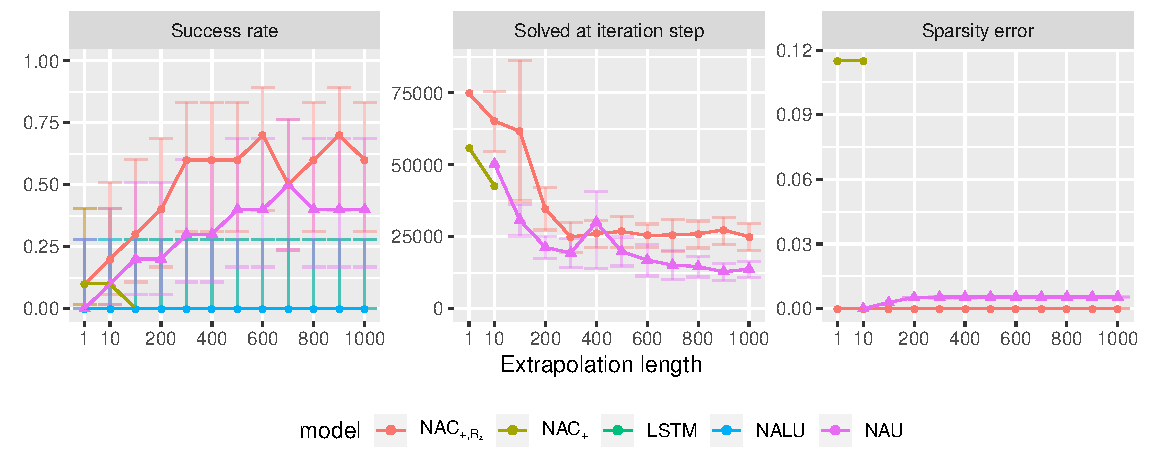
\includegraphics[width=\linewidth,trim={0 0.5cm 0 0},clip]{paper/results/sequential_mnist_sum_long_ablation.pdf}
\caption{Same as figure \ref{fig:sequential-mnist-sum}, but where the NAU model do not use the $\mathrm{R}_z$ regularizer.} 
\label{fig:sequential-mnist-sum-ablation}
\end{figure}

\subsection{Sequential multiplication without the \texorpdfstring{$\mathrm{R}_z$}{R\_z} regularizer}
\label{sec:appendix:sequential-mnist:ablation}

As an ablation study of the $\mathrm{R}_z$ regularizer figure \ref{fig:sequential-mnist-prod-ablation} shows the NMU and $\mathrm{NAC}_{\bullet,\mathrm{NMU}}$ models without the $\mathrm{R}_z$ regularizer. The success-rate is somewhat similar to figure \ref{fig:sequential-mnist-prod-results}. However, as seen in the ``sparsity error'' plot, the solution is quite different.

\begin{figure}[h]
\centering
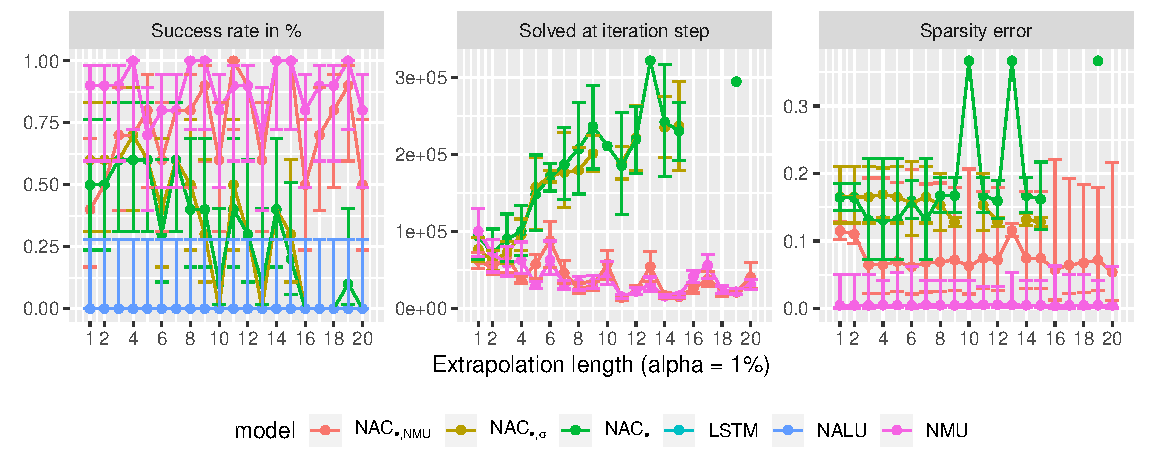
\includegraphics[width=\linewidth,trim={0 0.5cm 0 0},clip]{results/sequential_mnist_prod_long_ablation.pdf}
\caption{Shows the ability of each model to learn the arithmetic operation of addition and backpropagate through the arithmetic layer in order to learn an image-to-scalar value for MNIST digits. The model is tested by extrapolating to larger sequence lengths than what it has been trained on. The NMU and $\mathrm{NAC}_{\bullet,\mathrm{NMU}}$ models do not use the $\mathrm{R}_z$ regularizer.} 
\label{fig:sequential-mnist-prod-ablation}
\end{figure}